\documentclass[11pt]{beamer}
\usepackage{hyperref}
\usepackage[T1]{fontenc}
\UseRawInputEncoding

\usepackage{graphicx}
\usepackage[utf8]{inputenc}
\usepackage{mathtools}
\usepackage{verbatim}
\usepackage{smartdiagram}
\usepackage{unicode-math}
%\setmathfont{}
\usepackage{comment}
\usepackage{xcolor}
% Cannot enable in Xelatex
\usepackage{pgfpages}
% \setbeameroption{hide notes} % Only slides
% \setbeameroption{show only notes} % Only notes
% \setbeameroption{show notes on second screen}
\usepackage{latexsym,amsmath,xcolor,multicol,booktabs,calligra}
\usepackage{graphicx,listings,stackengine}

\usepackage{tikz}
\usepackage{tikz-feynman}
\usepackage[compat=1.0.0]{tikz-feynman}
\usepackage{float}

%% Enable only in Xelatex
% \usepackage{pstricks}
\usepackage{feynmp-auto} % or feynmp if you prefer
% Feynman diagrams
%\usepackage{feynmp}
%\usepackage{feynmf}
\DeclareGraphicsRule{*}{mps}{*}{} % for being able to read the produced file

\author{Ana Costa Pereira}
\title{$V_{ud}$ extraction from EW corrections}
\institute [University of Liverpool] {\href{mailto:Ana.Costa-Pereira@liverpool.ac.uk}{\underline{Ana.Costa-Pereira@liverpool.ac.uk}}}
\date{30/06/2026}
\usepackage{QUT}

% defs
\def\cmd#1{\texttt{\color{red}\footnotesize $\backslash$#1}}
\def\env#1{\texttt{\color{blue}\footnotesize #1}}
\definecolor{deepblue}{rgb}{0,0,0.5}
\definecolor{deepred}{rgb}{0.6,0,0}
\definecolor{deepgreen}{rgb}{0,0.5,0}
\definecolor{halfgray}{gray}{0.55}

\lstset{
    basicstyle=\ttfamily\small,
    keywordstyle=\bfseries\color{deepblue},
    emphstyle=\ttfamily\color{deepred},    % Custom highlighting style
    stringstyle=\color{deepgreen},
    numbers=left,
    numberstyle=\small\color{halfgray},
    rulesepcolor=\color{red!20!green!20!blue!20},
    frame=shadowbox,
}

\setbeamercolor{block body alerted}{bg=alerted text.fg!10}
\setbeamercolor{block title alerted}{bg=alerted text.fg!20}
\setbeamercolor{block body}{bg=structure!10}
\setbeamercolor{block title}{bg=structure!20}
\setbeamercolor{block body example}{bg=green!10}
\setbeamercolor{block title example}{bg=green!20}

\begin{document}
%
%
% Capa
%
%
\begin{frame}
    \titlepage

    \begin{columns}[c]
        \column{0.5\textwidth}
        \centering
        
\includegraphics[width=0.7\linewidth]{logo.png}

        \column{0.5\textwidth}
        \centering
        
\includegraphics[width=0.7\linewidth]{logo_livinno.jpg}
    \end{columns}
\end{frame}


\begin{frame}
    \tableofcontents[sectionstyle=show,subsectionstyle=show/shaded/hide,subsubsectionstyle=show/shaded/hide]
\end{frame}













\begin{frame}{Motivation and Overview}

\begin{itemize}
\item \textbf{CKM matrix} $\longrightarrow$ quark flavour mixing in weak interactions;
\vspace{0.2cm}

\item First-row unitarity test
\[
|V_{ud}|^2 + |V_{us}|^2 + |V_{ub}|^2 = 1,
\]
provides a sensitive probe of the SM;
%\vspace{0.2cm}

\item Current determinations of $V_{ud}$ and $V_{us}$ show a mild tension $\longrightarrow$ \textbf{Cabibbo Angle Anomaly};
%\vspace{0.2cm}

\item Precision measurements of weak decays and accurate theoretical inputs
are needed to clarify this tension;
%\vspace{0.2cm}

\item This talk:
\begin{itemize}
    \item Status of $V_{ud}$ from superallowed $\beta$ decays, pion decay and neutron decay;
    \item Ongoing work on \textbf{NNLO EW corrections for neutron decay} and $V_{ud}$ extraction.
\end{itemize}

\end{itemize}

\end{frame}












\section{CKM matrix}

\begin{frame}{CKM matrix}
\begin{figure}
    \centering
    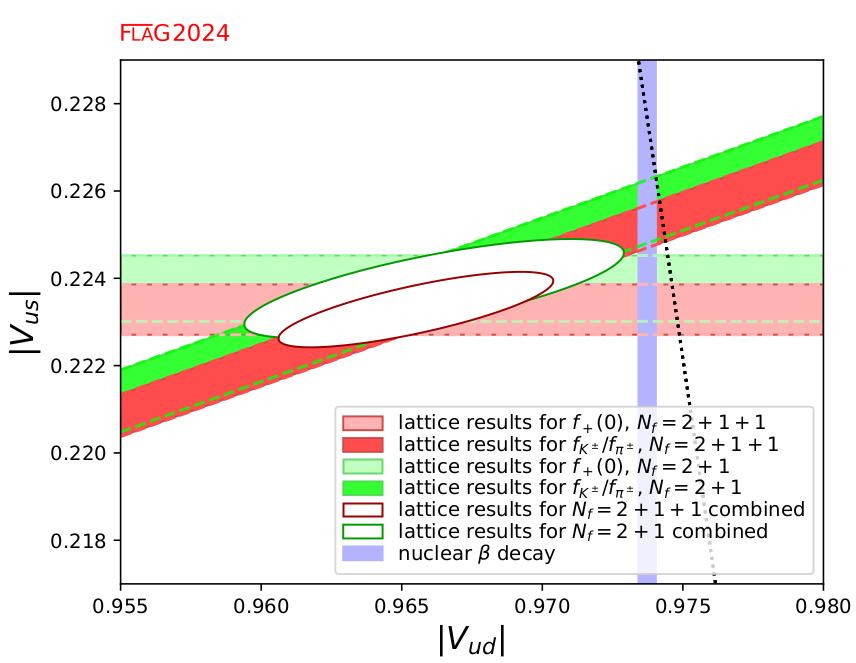
\includegraphics[scale=.25]{images/f.png}
\end{figure}

\centering
\footnotesize
$V_{ud}$ and $V_{us}$ using lattice QCD input and $V_{ud}$ extracted from nuclear $\beta$ decays, FLAG2024.
\end{frame}

















\section{$V_{ud}$ from neutron decay}

\begin{frame}{$V_{ud}$ from neutron decay}

\[
\frac{1}{\tau_n}
=
\frac{G_F^2 |V_{ud}|^2}{2\pi^3}
m_e^5 f (1+3g_A^2)(1+\Delta_R^V)
\]

\begin{itemize}
    \item $f$ phase-space factor
    \item $g_A$ axial coupling
    \item $\Delta_R^V$ universal electroweak radiative correction.
\end{itemize}

\[
\Delta_R^V = 2.436(16)\%
\]

\[
|V_{ud}|_n = 0.97410(41)
\]

\begin{itemize}
    \item First NLL calculation of mixed $O(\alpha\alpha_s^2)$ corrections;
    \item Reduced scale and scheme dependence;
    \item Improved CKM first-row unitarity tests;
\end{itemize}
{\footnotesize

\hyperref{https://arxiv.org/pdf/2510.27648}{Gorbahn, Jäger, Moretti (2025)}
}
\end{frame}














\section{$V_{ud}$ EFT framework}

\begin{frame}{$V_{ud}$ in the EFT framework}

\[
d \to u\,e\,\bar\nu_e
\]

\begin{columns}[c]

\begin{column}{0.45\textwidth}
\centering
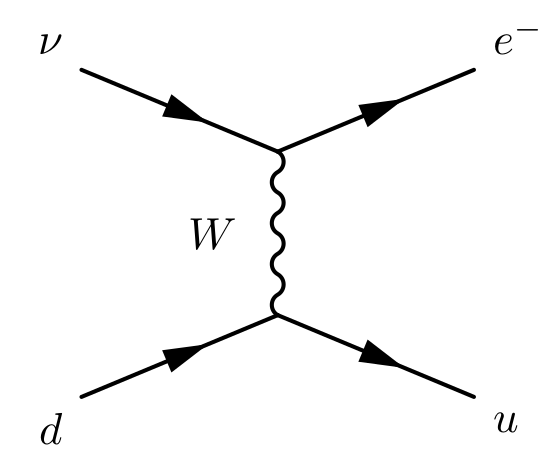
\includegraphics[width=0.8\textwidth]{images/full.png}

\vspace{0.2cm}
{\small Standard Model}
\end{column}

\begin{column}{0.1\textwidth}
\centering
\[
m_W \gg k
\]

\[
\Longrightarrow
\]
\end{column}

\begin{column}{0.45\textwidth}
\centering
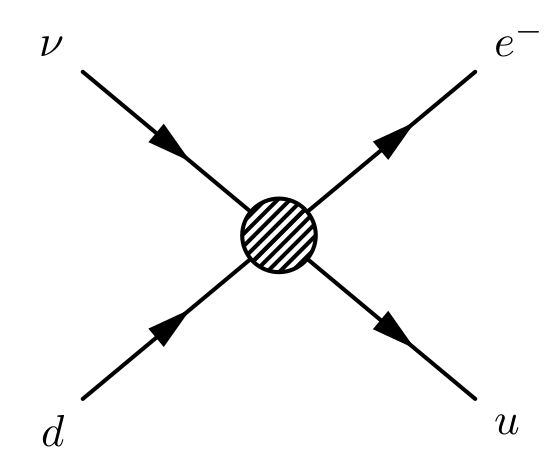
\includegraphics[width=0.8\textwidth]{images/eft.png}

\vspace{0.2cm}
{\small Effective theory}
\end{column}

\end{columns}

%\vspace{0.3cm}

%\[
%\frac{1}{k^2-m_W^2}
%=
%-\frac{1}{m_W^2}
%+\mathcal O\!\left(\frac{k^2}{m_W^4}\right)
%\]

\vspace{0.2cm}

\[
\mathcal H_{\rm eff}
=
\frac{G_F}{\sqrt2}
V_{ud}\,
C_q(\mu)\,
Q_q
\]

\end{frame}











\begin{frame}{Physical and Evanescent operators}
\small
    \begin{equation*}
    Q_1 = (\Bar{d} \gamma^{\mu} P_L u ) (\Bar{\nu} \gamma^{\mu} P_L e ) 
\end{equation*}

\begin{equation*}
      E_1 = (\overline{d} \gamma^\mu \gamma^\nu \gamma^\beta P_L u )(\overline{\nu}\gamma_\mu \gamma_\nu \gamma_\beta P_L e)
      - (16- a_q^1 \epsilon - a_q^2 \epsilon^2)  Q_1
\end{equation*}


\begin{equation*}
      E_2 = (\overline{d} \gamma^\mu \gamma^\nu \gamma^\alpha \gamma^\beta \gamma^\sigma P_L u )(\overline{\nu}\gamma_\mu \gamma_\nu \gamma_\alpha \gamma_\beta \gamma_\sigma P_L e)
      - (256 - b^1_{q} \epsilon - b^2_{q} \epsilon^2 )  Q_1 + c^0_{q} E_1
\end{equation*}

\begin{itemize}
\item d dimensions (vanish in 4 dimensions);
\item scheme dependent;
\end{itemize}

\end{frame}











\begin{frame}{Guide for amplitude computation}
\centering
    Generate the diagrams with the SM\\
$\downarrow$\\
    Compute the amplitudes $\longrightarrow$ tensor integrals $\longrightarrow$ tensor decomposition $\longrightarrow$ reduction to masters\\
$\downarrow$\\
analytical amplitudes\\
$\downarrow$\\
    $\overline{MS}$ renormalization $\longrightarrow$ renormalized amplitude
    \\
    \vspace{.5cm}
    \textbf{Choice of kinematics:} external momenta set to zero and all masses bellow the W mass are set to zero. Only masses present in our calculation will be $m_W$, $m_Z$, $m_H$, $m_t$. 
\end{frame}












\section{NLO EW corrections}



\begin{frame}{EFT and Infrared Rearrangement}
\centering
\footnotesize 1 loop EFT contribution for pion decay.
\begin{figure}
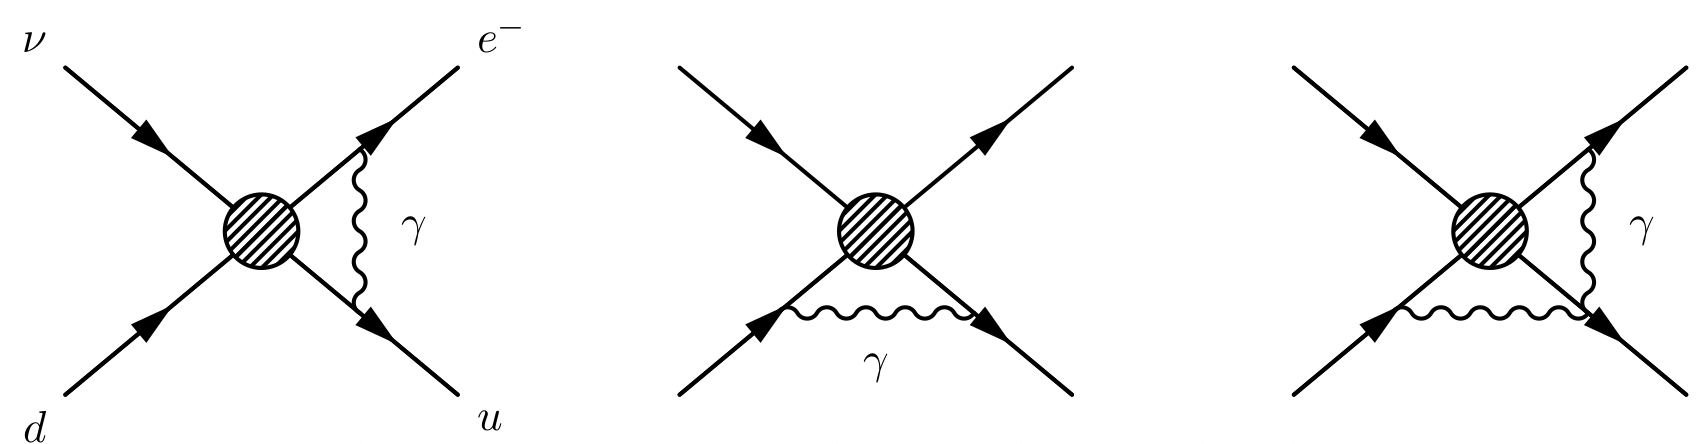
\includegraphics[scale=.15]{images/eft1l.png}
\end{figure}
\vspace{0.2cm}
Exact decomposition of a propagator

\begin{equation*} \label{IR rearr}
    \dfrac{1}{(k+p)^2-m^2} = \dfrac{1}{k^2-M^2} + \frac{-p^2+ 2 k \cdot p -m^2 + M^2}{k^2-M^2} \frac{1}{(k+p)^2 - m^2}
\end{equation*}

 $k$ and $p$ stand for a linear combination of the internal moment and external momenta. The propagator mass is $m$ and $M$ is an introduced fictitious regulator. 
\end{frame}












\begin{frame}{NLO EW corrections}

\textbf{Matching condition}
\[
\mathcal A_{\rm SM}
=
\mathcal A_{\rm EFT} = V_{ud} C_q Q_q
\]

\begin{figure}
\centering

%----------------------------------------------------
% Diagram 1
%----------------------------------------------------
\begin{minipage}{0.23\textwidth}
\centering
\begin{tikzpicture}[scale=0.65, transform shape]
\begin{feynman}
\vertex (u) at (0,1.5) {\(u\)};
\vertex (a) at (1.5,1.5);
\vertex (d) at (3,1.5) {\(d\)};
\vertex (c1) at (1.5,0.975);
\vertex (c2) at (1.5,0.525);
\vertex (c) at (1.5,0);
\vertex (e) at (0,0) {\(e\)};
\vertex (ve) at (3,0) {\(\nu_e\)};
\diagram* {
  (u) -- [fermion] (a) -- [fermion] (d),
  (a) -- [boson, edge label=\(W\)] (c1),
  (c1) -- [fermion, half left, looseness=1.4, edge label=\(b\)] (c2)
        -- [fermion, half left, looseness=1.4, edge label=\(t\)] (c1),
  (c2) -- [boson, edge label=\(W\)] (c),
  (e) -- [fermion] (c) -- [fermion] (ve),
};
\end{feynman}
\end{tikzpicture}
\end{minipage}
\hfill
%----------------------------------------------------
% Diagram 2
%----------------------------------------------------
\begin{minipage}{0.23\textwidth}
\centering
\begin{tikzpicture}[scale=0.65, transform shape]
\begin{feynman}
\vertex (u) at (0,1.5) {\(u\)};
\vertex (a) at (1,1.5);
\vertex (a1) at (2,1.5);
\vertex (d) at (3,1.5) {\(d\)};
\vertex (e) at (0,0) {\(e\)};
\vertex (c) at (1,0);
\vertex (c1) at (2,0);
\vertex (ve) at (3,0) {\(\nu_e\)};
\diagram* {
  (u) -- [fermion] (a) -- [fermion, edge label=\(u\)] (a1) -- [fermion] (d),
  (a) -- [boson, edge label'=\(Z\)] (c),
  (a1) -- [boson, edge label=\(W\)] (c1),
  (e) -- [fermion] (c) -- [fermion, edge label'=\(e\)] (c1)
      -- [fermion] (ve),
};
\end{feynman}
\end{tikzpicture}
\end{minipage}
\hfill
%----------------------------------------------------
% Diagram 3
%----------------------------------------------------
\begin{minipage}{0.23\textwidth}
\centering
\begin{tikzpicture}[scale=0.65, transform shape]
\begin{feynman}
\vertex (u) at (0,1.5) {\(u\)};
\vertex (a) at (1,1.5);
\vertex (a1) at (2,1.5);
\vertex (d) at (3,1.5) {\(d\)};
\vertex (e) at (0,0) {\(e\)};
\vertex (c) at (1.5,0);
\vertex (c1) at (1.5,0.6);
\vertex (ve) at (3,0) {\(\nu_e\)};
\diagram* {
  (u) -- [fermion] (a) -- [fermion, edge label=\(d\)] (a1) -- [fermion] (d),
  (a) -- [boson, edge label'=\(W\)] (c1),
  (a1) -- [boson, edge label=\(\gamma\)] (c1),
  (c1) -- [boson, edge label=\(W\)] (c),
  (e) -- [fermion] (c) -- [fermion] (ve),
};
\end{feynman}
\end{tikzpicture}
\end{minipage}
\hfill
%----------------------------------------------------
% Diagram 4
%----------------------------------------------------
\begin{minipage}{0.23\textwidth}
\centering
\begin{tikzpicture}[scale=0.65, transform shape]
\begin{feynman}
\vertex (u) at (0,1.5) {\(u\)};
\vertex (a) at (1.5,1.5);
\vertex (d) at (3,1.5) {\(d\)};
\vertex (c1) at (1.5,0.75);
\vertex (c2) at (2,0.75);
\vertex (c3) at (2.4,0.75);
\vertex (c) at (1.5,0);
\vertex (e) at (0,0) {\(e\)};
\vertex (ve) at (3,0) {\(\nu_e\)};
\diagram* {
  (u) -- [fermion] (a) -- [fermion] (d),
  (a) -- [boson, edge label'=\(W\)] (c),
  (c1) -- [scalar, edge label=\(H\)] (c2)
        -- [fermion, half left, looseness=1.4] (c3)
        -- [fermion, half left, looseness=1.4, edge label=\(W\)] (c2),
  (e) -- [fermion] (c) -- [fermion] (ve),
};
\end{feynman}
\end{tikzpicture}
\end{minipage}
\scriptsize Representative one-loop EW diagrams contributing to the semi-leptonic process.
\end{figure}

\small

\begin{columns}[c]

\begin{column}{0.48\textwidth}

\textbf{Wilson coefficient}

\[
C_q(\mu)
=
1+
\frac{\alpha}{4\pi}
\,C_q^{\rm NLO}
+
(\frac{\alpha}{4\pi})^{2}
\,C_q^{\rm NNLO}
\]

\[
C_q^{\rm NLO}
=
-5 +\frac{a_\mu^1}{4}+\frac{a_q^1}{12}
-
2\ln\!\left(\frac{\mu^2}{M_Z^2}\right)
\]

\end{column}

\begin{column}{0.48\textwidth}

\begin{itemize}
\item Matching performed at the electroweak scale.

\item Universal corrections cancel in the ratio of the quark decay normalized to muon decay: $\frac{C_q}{C_\mu}.$

\item Only box-diagram contributions survive.
\end{itemize}

\end{column}

\end{columns}
\end{frame}














\section{NNLO EW corrections}
\begin{frame}{NNLO EW corrections}
\begin{figure}
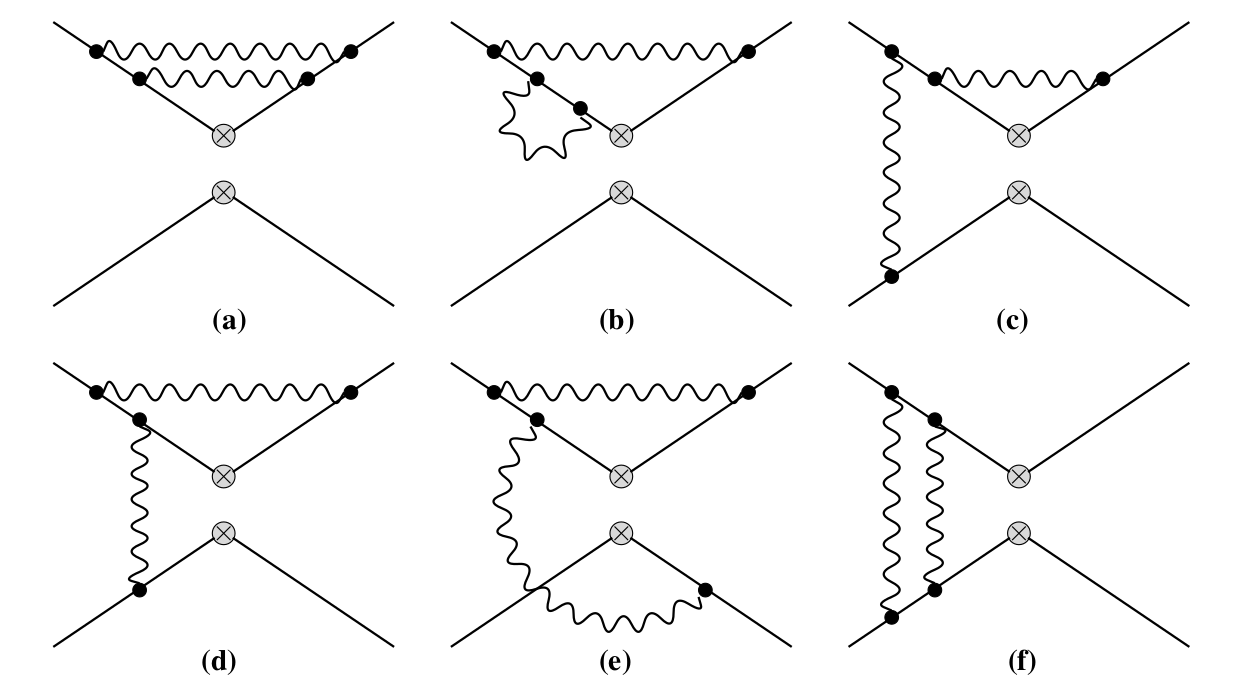
\includegraphics[scale=.13]{images/eft2l.png}
\scriptsize
EFT NNLO EW corrections.
\end{figure}
\begin{figure}
\centering

%---------------- First row ----------------
\begin{minipage}{0.16\textwidth}
\centering
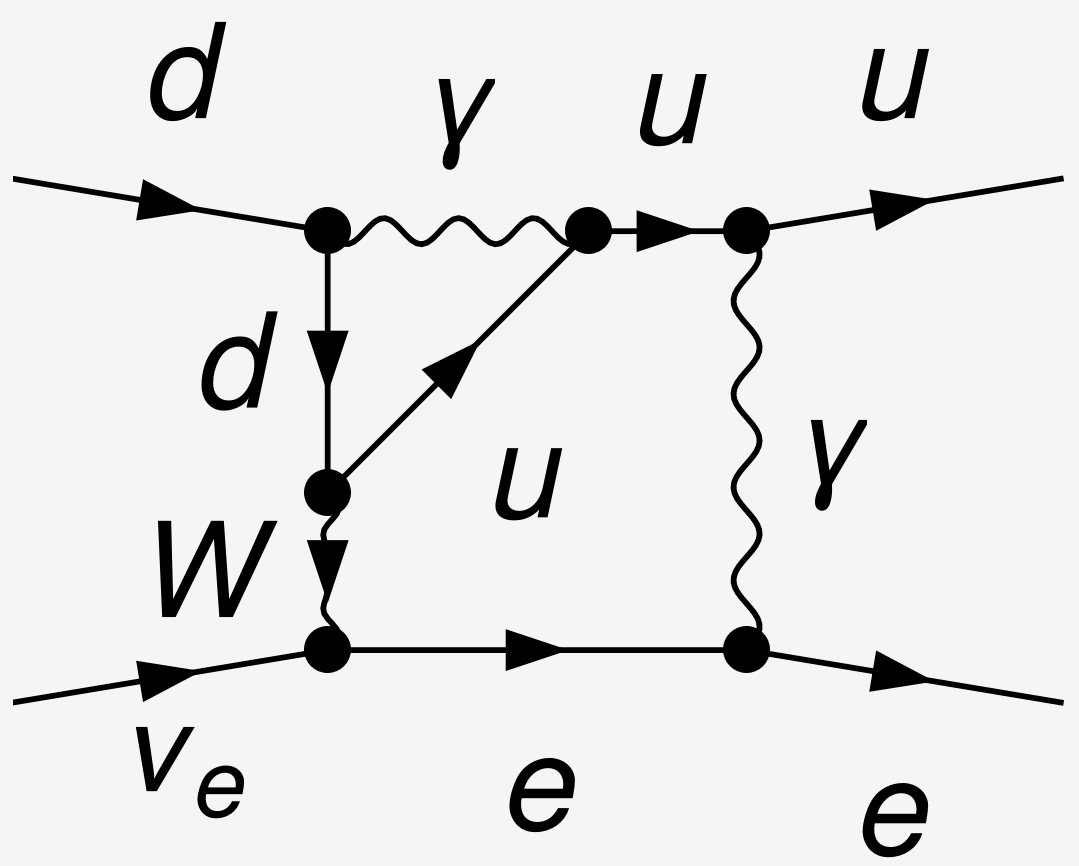
\includegraphics[width=\linewidth]{images/bb1.png}
\end{minipage}
\hfill
\begin{minipage}{0.16\textwidth}
\centering
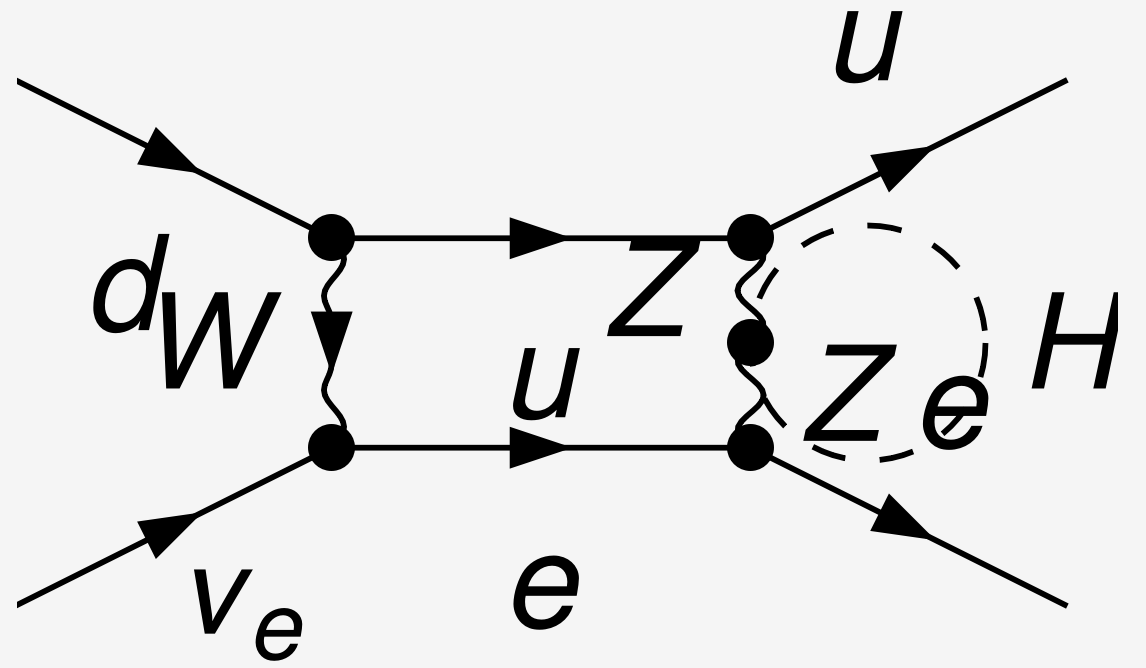
\includegraphics[width=\linewidth]{images/bb2.png}
\end{minipage}
\hfill
\begin{minipage}{0.16\textwidth}
\centering
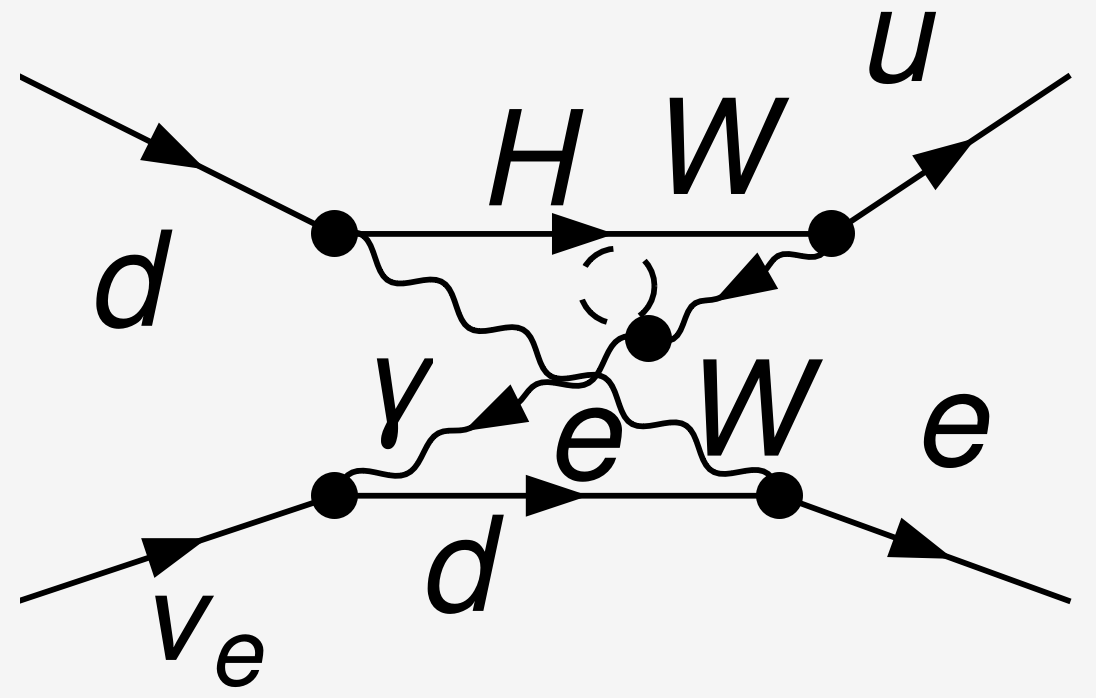
\includegraphics[width=\linewidth]{images/bb3.png}
\end{minipage}
\hfill
\begin{minipage}{0.16\textwidth}
\centering
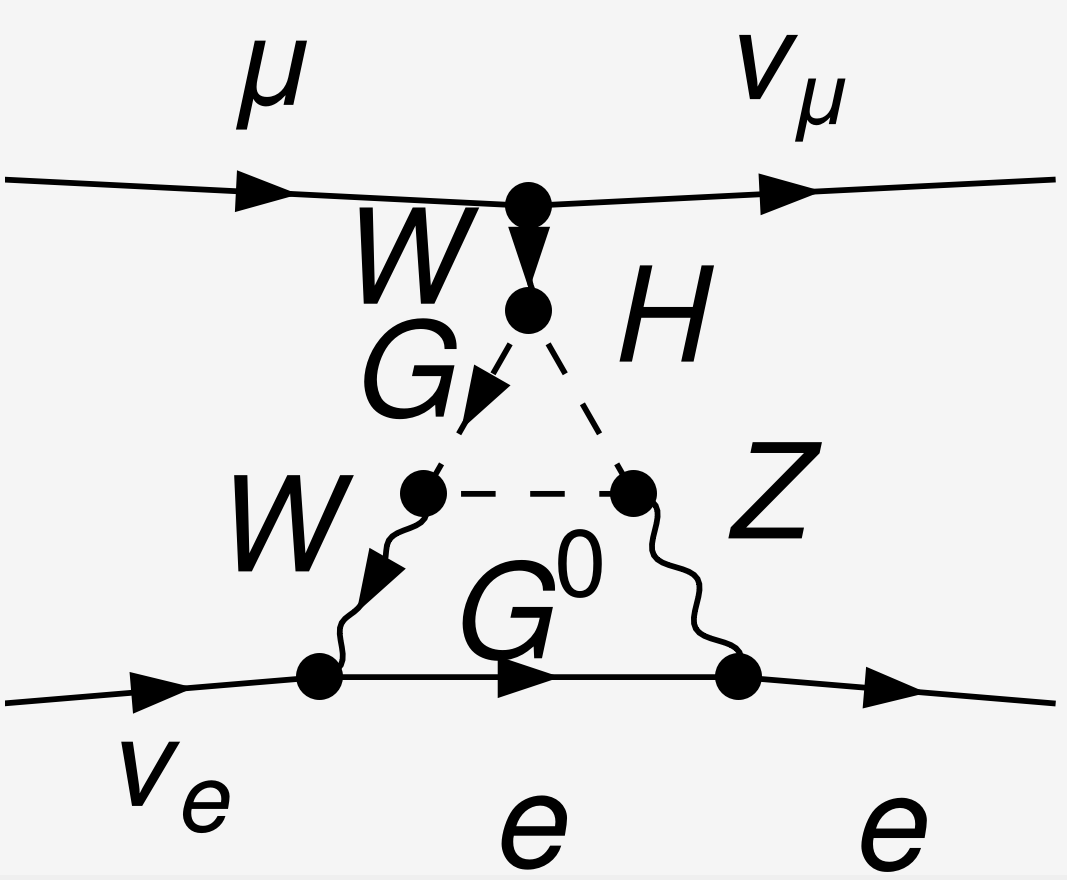
\includegraphics[width=\linewidth]{images/p1.png}
\end{minipage}
\hfill
\begin{minipage}{0.16\textwidth}
\centering
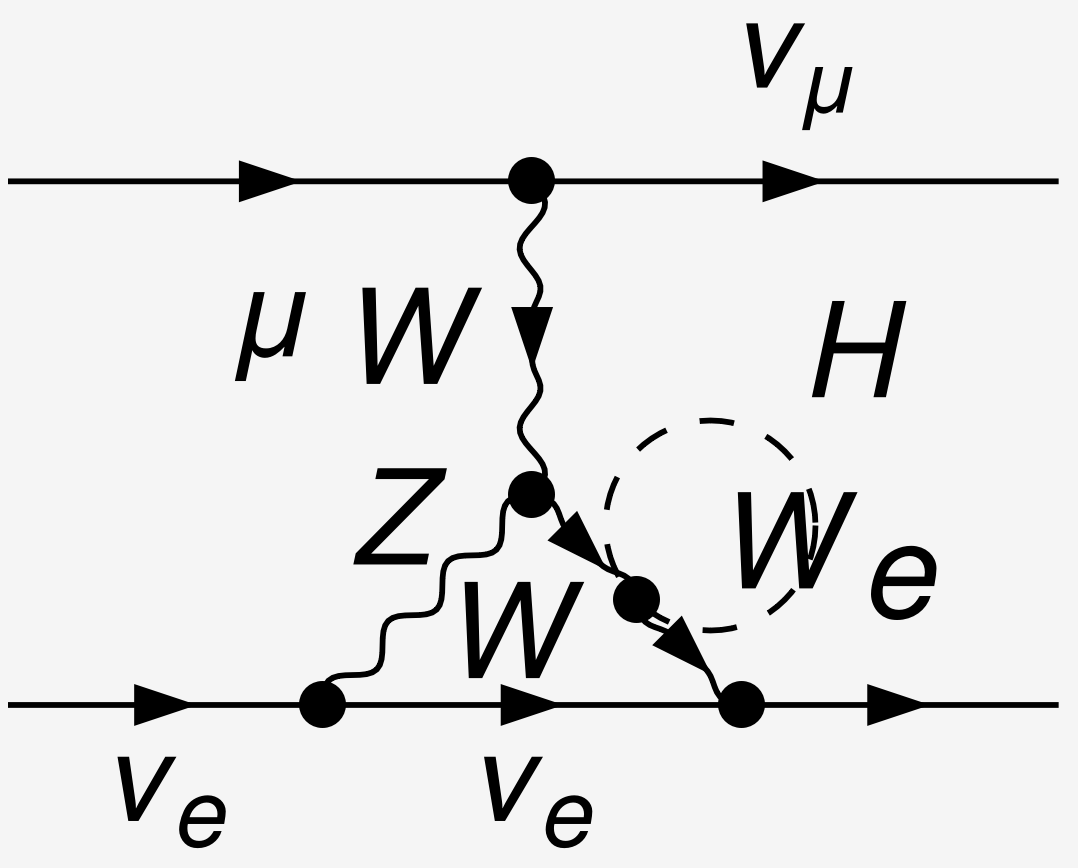
\includegraphics[width=\linewidth]{images/p2.png}
\end{minipage}

\scriptsize
SM NNLO EW corrections.
\end{figure}
\begin{itemize}
\item NNLO requires inclusion of boxes and penguins
\item Tadpoles are included in the matching: gauge independent NNLO EW corrections and potentially substancial contribution in scheme conversion: $\overline{MS}$ to On-Shell.
\end{itemize}
\end{frame}











\begin{frame}{WC and RGE}
WC depends on $\mu$:

\begin{equation}
\mu \frac{d}{d\mu} C^f_i(\mu)
=
\sum_j \gamma^f_{ij} \, C^f_j(\mu),
\end{equation}

\begin{itemize}
depends on active number of flavours;
\end{itemize}

Anomalous dimension for muon decay (physical operator)
\begin{align}
  \gamma^{(0)}_\mu &= 0\,,  & &
  \gamma^{(1)}_\mu =
   \left( \frac{2}{3} N_\ell
    +\frac{8}{27} n_c N_u
    +\frac{2}{27} n_c N_d
   \right)(4-a^1_\mu)
  \,,\\
  \gamma^{(0)}_q   &= -4\,, & &
  \gamma^{(1)}_q = 
        \left(
          \frac{16}{9} N_\ell
         +\frac{64}{81} n_c N_u
         +\frac{16}{81} n_c N_d
         \right)(a_q^1-8)
  \,.
\end{align}

\end{frame}










\begin{frame}{Scheme independence}
Solution of Renormalization Group Equations for the Wilson Coefficient

\begin{equation}
C^{(f)}(\mu)
=
J_f(\mu)\,
U_f(\mu)\,
U_f^{-1}(\mu_0)\,
J_f^{-1}(\mu_0)\,
C^{(f)}(\mu_0)
\end{equation}

Evolution kernel at LO

\begin{equation}
U_f(\mu)
=
\left(
\frac{\alpha^{(f)}(\mu)}
{\alpha(M_Z)}
\right)^{-\frac{\gamma^{(0)}}{2 \beta^{(0)}}}
\end{equation}

scheme independence

\begin{equation}
C = U_f^{-1}(\mu_0)\,
J_f^{-1}(\mu_0)\,
C^{(f)}(\mu_0)
\end{equation}

\end{frame}












\begin{frame}{Wilson-Coefficient residual scale dependence}

\centering
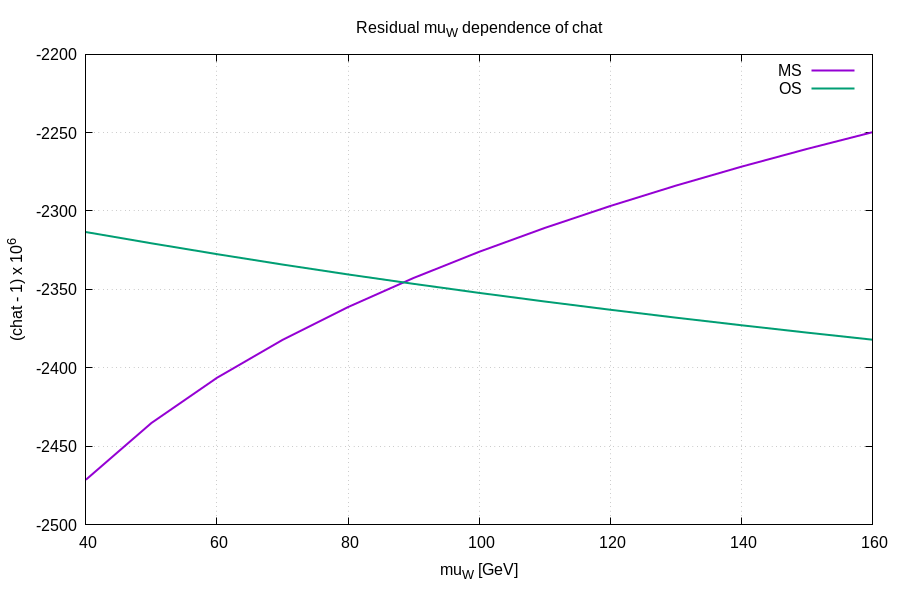
\includegraphics[scale=.22]{images/chat_muw_scan.png}

\vspace{0.2cm}
\scriptsize
Scale dependence of the scale independent Wilson coefficient at NLO.

\vspace{0.4cm}

\begin{itemize}
\item Residual scale dependence at NLO induces an uncertainty
$\delta C \simeq \pm 2\times10^{-4}$,
which is significant for precision determinations of $V_{ud}$.

\item NNLO corrections reduce the uncertainty to
$\delta C < 2\times10^{-5}$,
making perturbative uncertainties essentially negligible.
\end{itemize}

\end{frame}











\begin{comment}

\begin{frame}
\begin{figure}

\includegraphics[scale=.15]{eft2l.png}
\caption{EFT NNLO EW corrections.}
\end{figure}
\begin{figure}[h]
\centering

\begin{minipage}{0.48\textwidth}
\centering
\begin{tikzpicture}
\begin{feynman}
\vertex (u) at (0,1.5) {\(u\)};
\vertex (a) at (1,1.5);
\vertex (a1) at (2,1.5);
\vertex (a2) at (3,1.5);
\vertex (d) at (4,1.5) {\(d\)};

\vertex (e) at (0,0) {\(e\)};
\vertex (c) at (1,0);
\vertex (c1) at (2,0);
\vertex (c2) at (3,0);
\vertex (ve) at (4,0) {\(\nu_e\)};

\diagram* {
  (u) -- [fermion] (a) -- [fermion, edge label=\(u\)] (a1) -- [fermion, edge label=\(u\)] (a2) -- [fermion] (d),
  (a) -- [boson, edge label'=\(Z\)] (c),
  (a1) -- [boson, edge label=\(Z\)] (c1),
  (a2) -- [boson, edge label=\(W\)] (c2),
  (e) -- [fermion] (c) -- [fermion, edge label'=\(e\)] (c1)
      -- [fermion, edge label'=\(e\)] (c2) -- [fermion] (ve),
};
\end{feynman}
\end{tikzpicture}

\end{minipage}
\hfill
\begin{minipage}{0.48\textwidth}
\centering
\begin{tikzpicture}
\begin{feynman}
\vertex (u) at (0,1.5) {\(u\)};
\vertex (a) at (1,1.5);
\vertex (a1) at (2,1.5);
\vertex (d) at (3,1.5) {\(d\)};
\vertex (a2) at (1.3,1);
\vertex (a3) at (1.7,1);

\vertex (e) at (0,0) {\(e\)};
\vertex (c) at (1.5,0);
\vertex (c1) at (1.5,0.4);
\vertex (ve) at (3,0) {\(\nu_e\)};

\diagram* {
  (u) -- [fermion] (a) -- [fermion, edge label=\(u\)] (a1) -- [fermion] (d),
  (a) -- [boson, edge label'=\(\gamma\)] (a2) -- [fermion, edge label'=\(e\)] (c1),
  (a1) -- [boson, edge label=\(W\)] (a3) -- [fermion, edge label=\(\nu_e\)] (c1),
  (a2) -- [fermion, edge label=\(e\)] (a3),
  (c1) -- [boson, edge label=\(W\)] (c),
  (e) -- [fermion] (c) -- [fermion] (ve),
};
\end{feynman}
\end{tikzpicture}


\end{minipage}

\caption{SM NNLO EW corrections.}
\end{figure}
\end{frame}
\end{comment}

















\begin{frame}{Conclusions}
    \begin{itemize}
        \item Combination of lattice inputs and perturbative calculations;
        \item Higher order calculation + sub-percent lattice calculations;
        \item Current ongoing work on NNLO EW corrections for $V_{ud}$ extraction from neutron decay. 
    \end{itemize}
\end{frame}






\begin{frame}{Parallel scaling at higher thread count}
\begin{figure}
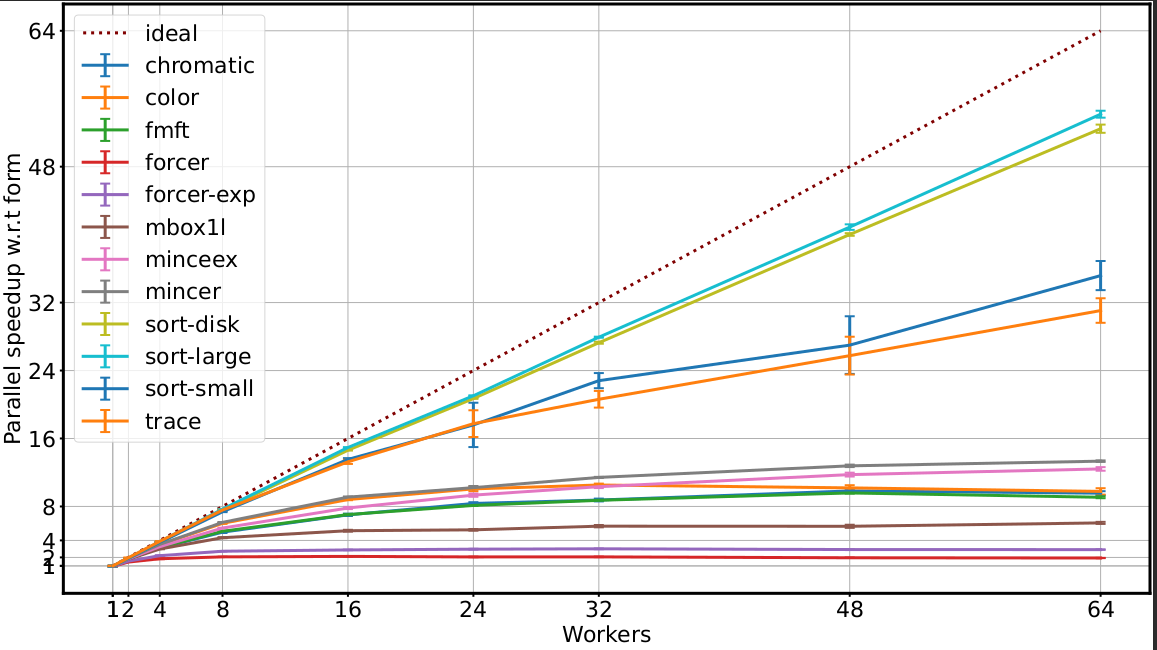
\includegraphics[scale=.20]{images/plotparallel.png}
\end{figure}
\begin{itemize}
\item sort-disk, sort-large, sort-small, trace scale up to 64;
\item scaling is not good for other tests for $>16$ \textcolor{orange}{workers}.
\end{itemize}
\end{frame}










%\section{SortBot Merging}


\begin{frame}{SortBot Merging}
\small
\begin{itemize}
\item \textcolor{magenta}{Master} $\longrightarrow$ distributes terms to the workers;
\item \textcolor{orange}{Worker} $\longrightarrow$ independent stream of sorted terms;
\item  $N$ \textcolor{orange}{workers} $\longrightarrow$ $N-2$ \textcolor{blue}{SortBots} are created; 
\item \textcolor{blue}{SortBot} routine starts; 
\end{itemize}
\begin{figure}
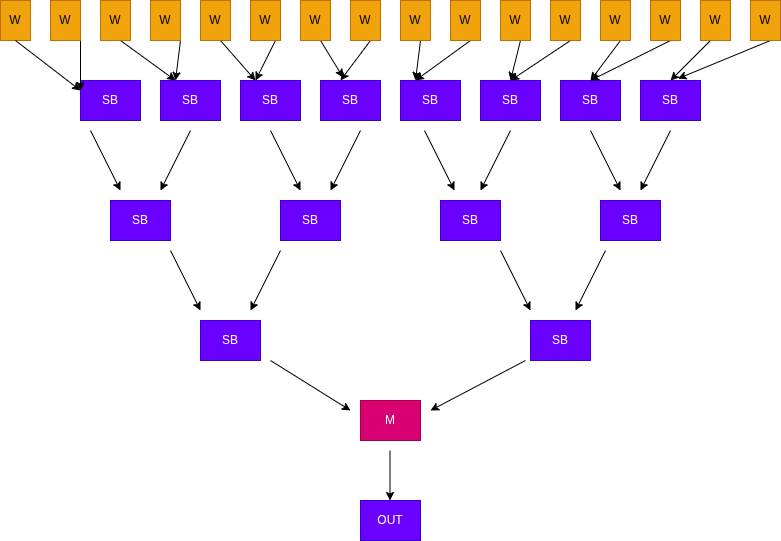
\includegraphics[scale=.20]{images/sb.png}
\end{figure}
\begin{itemize}
    \item \textcolor{magenta}{Master} performs the final merge and writes output.
\end{itemize}
\end{frame}














%\section{SortBot Bottlenecks and changes}

\begin{frame}{SortBot: Overlaping of terms}
\begin{itemize}
\item \textcolor{blue}{SortBot} $\longrightarrow$ ring buffer with blocks;
\end{itemize}
\begin{figure}
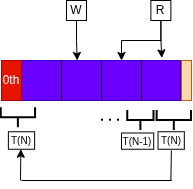
\includegraphics[scale=.50]{images/sb5.png}
\end{figure}
\begin{itemize}
\item Terms are allowed to overlap between blocks;
\item \textcolor{red}{0th block} - the overlap in the end of term is copied to \textcolor{red}{0th block} so that the terms are contiguous.
\end{itemize}
\end{frame}












\begin{frame}{SortBlocks Bottlenecks}
\begin{itemize}
\item \textbf{Bottlenecks}: reading of the input with
\textbf{division of terms} from \textcolor{orange}{workers} to \textcolor{blue}{SortBlocks}; inverse tree at the end with the
\textbf{writing to the file by the \textcolor{magenta}{Master}};
\end{itemize}
\begin{figure}
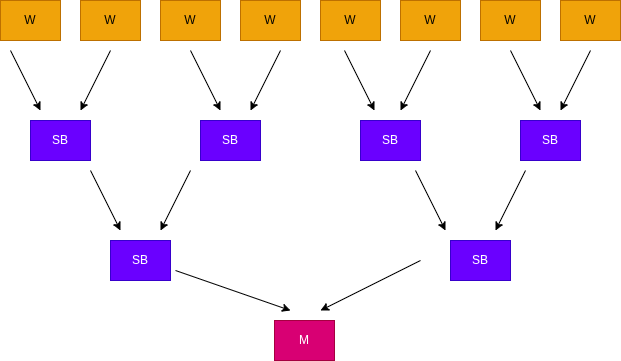
\includegraphics[scale=.3]{images/sb6.png}
\end{figure}
\end{frame}













\begin{frame}
\textbf{Bottlenecks}
\begin{figure}
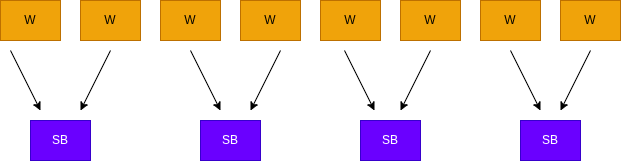
\includegraphics[scale=.30]{images/sb7.png}
\end{figure}
\begin{itemize}
\item Default buffer size increased over time$\longrightarrow$ bigger \textcolor{blue}{SortBlocks}; 
\item Result from \textcolor{orange}{worker} fits into \textbf{single block} $\longrightarrow$ SortBotTree mechanism does not parallelize
\item If a \textbf{term} does not fit at the end of a block: Writer fills the \textcolor{blue}{SortBlocks} all the way up to the end of the block, \textbf{overlapping} to the next;
\item Once a block is completely full, it reaches the top and moves on to the next block.
\end{itemize}
\end{frame}














%\section{Changes in the SortBot Merge}

\begin{frame}{Change: SortBot Block size}
\begin{figure}
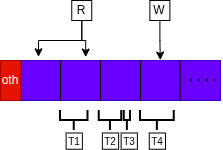
\includegraphics[scale=.5]{images/sb8.png}
\end{figure}
\begin{itemize}
\item Require fewer \textcolor{blue}{SortBlocks} - master buffers not expanded so often;
\item Whole terms must fit into the block: if it does not fit, it goes into the next block;
\end{itemize}
\end{frame}











%\section{SortBot Locking}
\begin{frame}{Locking}
\begin{figure}
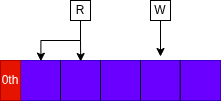
\includegraphics[scale=.50]{images/sb3.png}
\end{figure}
\begin{itemize}
\item Reading thread always locks pair of blocks - the current one and the previous;
\item Writing thread locks the block where it is writing;
\end{itemize}
\end{frame}















\begin{frame}{Change: SortBot Locking}
\begin{figure}
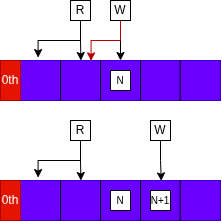
\includegraphics[scale=.50]{images/sb4.png}
\end{figure}
\begin{itemize}
\item Writer (W) detects if there is a Reader (R) waiting for it;
\item W filling the blocks tries to obtain a lock of the block before the current fill block;
\item If W does not obtain the lock, R thread already has the lock - very soon will be done and ready for more terms;
\item The W moves to the next block;
\end{itemize}
\end{frame}






\begin{frame}{SortBot variables}
\begin{itemize}
\item The number of blocks in each \textcolor{blue}{SortBot} has to be at least 4 (due to the locking mechanism) - which corresponds to a minimum of 8 for \textbf{NUMBEROFBLOCKSINSORT};
\item There is a minimum number of terms that have to fit the block: \textbf{MINNUMBEROFTERMS};
\item Make sure a minimum number of terms is written: never make empty block - \textbf{MINWRITENUMBEROFTERMS};
\end{itemize}
\end{frame}








\begin{frame}{Final result}
\href{https://github.com/form-dev/form/pull/831}{PR \#831}

\begin{itemize}
\item \textbf{NUMBEROFBLOCKSINSORT} = 10 $\longrightarrow$ 8
\item \textbf{MINNUMBEROFTERMS} = 10 $\longrightarrow$ 1
\item \textbf{MINWRITENUMBEROFTERMS} = 1
\end{itemize}
\begin{figure}
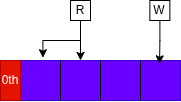
\includegraphics[scale=.5]{images/sb9.png}
\end{figure}
\end{frame}










\begin{frame}{Results after changes}
\begin{itemize}
\item No decrease in performance for any tests;
\item Performance improvement for benchmarks where term merging is expensive (PolyRatFun, PolyRatFunExpand)
\item Forcer, mbox1l
\end{itemize}
\end{frame}








\begin{frame}{Results after changes: Profiler}
\begin{itemize}
\item Profiler: AMDuProf with 4 workers;
\item Test: generate a large number of terms, mostly sorting them;
\item Green: Masters/threads in activity;
\item Red: Master using \textbf{PutOut};
\end{itemize}
\begin{figure}
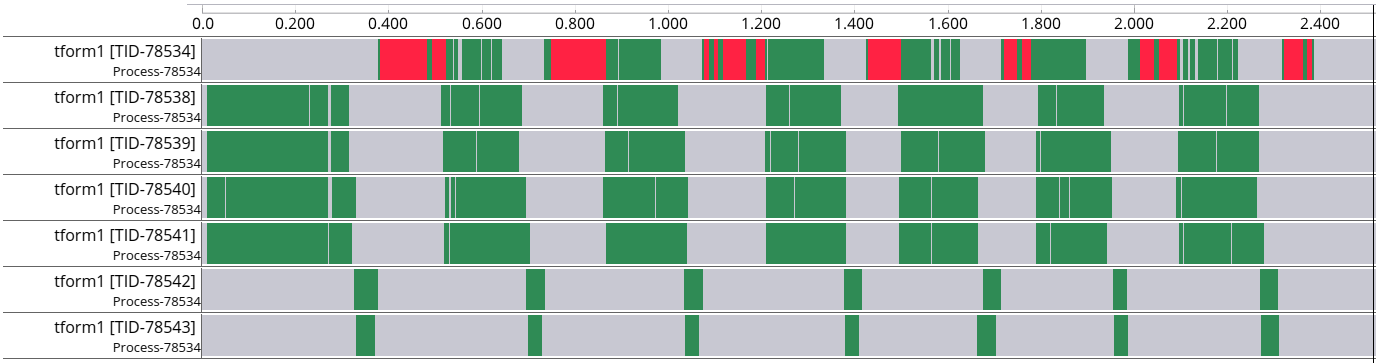
\includegraphics[scale=.2]{images/sbform1.png}
\end{figure}
\begin{figure}
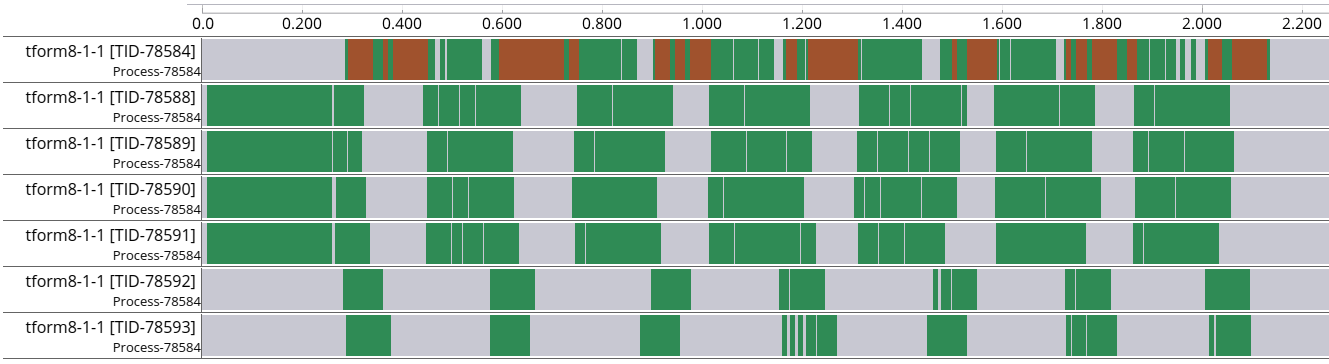
\includegraphics[scale=.2]{images/sbform8-1-1.png}
\end{figure}
\end{frame}










\begin{frame}{SortBlocks Bottlenecks}
\textbf{Bottlenecks}
\begin{figure}
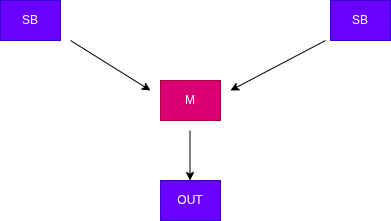
\includegraphics[scale=.30]{images/sb1.png}
\end{figure}
\begin{itemize}
\item End of the tree: \textcolor{magenta}{Master} performs last sorting as well as writing of terms into the output;
\item Performance could be increased by having one last stage of sorting of the last 2 \textcolor{blue}{SortBlocks} and \textcolor{magenta}{Master} only writing;
\end{itemize}
\end{frame}








\begin{frame}{Future Work: Addition of new SortBot}
\begin{itemize}
\item Add a new \textcolor{blue}{SortBot} at the end of the merging tree to sort the streams that come from last 2 \textcolor{blue}{SortBlocks};
\item \textcolor{magenta}{Master} only does the writing.
\end{itemize}
\begin{figure}
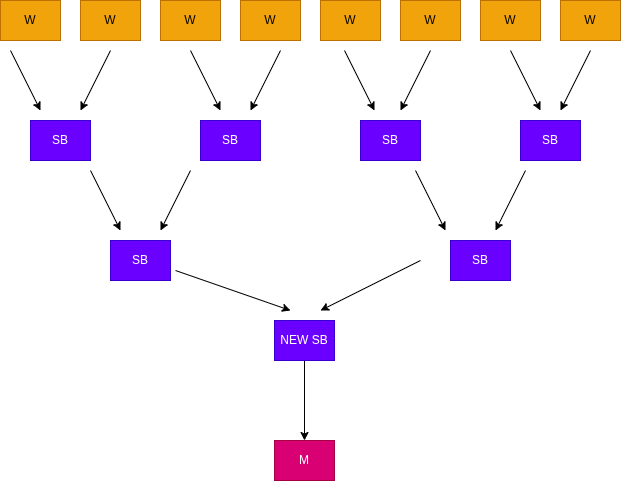
\includegraphics[scale=.3]{images/sb10.png}
\end{figure}
\end{frame}






\begin{frame}{Final remarks}
\begin{itemize}
\item Parallel performance at higher thread needs to be improved;
\item \textcolor{blue}{SortBot} changes - up to $30\%$ improvement for some tests;
\item Current working on improving \textcolor{blue}{SortBot} parallelization by addition of extra \textcolor{blue}{SortBot} at the end of the tree.
\end{itemize}
\end{frame}






\small
    \bibliographystyle{apalike}
%\printbibliography
\bibliography{slide}
\begin{comment}

\begin{frame}{Physical and Evanescent operator}
        In our case the relevant operators for the pion decay are a physical operator $Q(x)$

\begin{equation}
    Q(x) = (\Bar{d}(x) \gamma^{\mu} P_L u(x) ) (\Bar{\nu}(x) \gamma^{\mu} P_L e(x) ),     \space P_L = \dfrac{1 - \gamma_5}{2}
\end{equation}
\\
and an evanescent operator that can be related with the physical operator

\begin{equation}
E(x) = (\overline{d}(x) \gamma^\mu \gamma^\nu \gamma^\beta P_L u(x)) (\overline{\nu}(x) \gamma_\mu \gamma_\nu \gamma_\beta P_L l(x))
      - (16- a^1_q)  Q(x)
\end{equation}
which vanishes in 4 dimension.
\end{frame}

\begin{frame}{Results for the 1-loop EFT EW corrections for the semi-leptonic decay}
    The sum of the amplitudes $M$ of the 1-loop diagrams of the EFT 
\begin{equation}
    M_{EFT} = \int_k \frac{1}{(k^2-\mu^2)^2}(a_1 Q + a_2 E)
\end{equation}

with 

\begin{equation*}
\begin{split}
   &  a_1 = 
    \frac{\alpha}{4 \pi} G_F \Bigg( Q_u Q_d (\frac{(2-d)^2}{d} - (1 - \xi)) +
     Q_u Q_e (\frac{16}{d} - (1 - \xi))\\
     & + 
     Q_d Q_e (\frac{6d-20}{d} - (1 - \xi)) \Bigg)
\end{split}
\end{equation*}

\begin{equation*}
    a_2 = \frac{\alpha}{4 \pi} \frac{G_F}{d} \Big( Q_u Q_e - Q_d Q_e \Big)
\end{equation*}

with $Q_u$, $Q_d$, $Q_e$ being respectively the quark up, down and electron charges, $\alpha = \frac{e^2}{4 \pi}$ and $\xi$ is the Gauge of the photon.
\end{frame}

\begin{frame}{Infrared Rearrangement}
    The exact decomposition of a propagator which can be done in the following way

\begin{equation} \label{IR rearr}
    \dfrac{1}{(k+p)^2-m^2} = \dfrac{1}{k^2-\mu^2} + \frac{-p^2+ 2 k \cdot p -m^2 + \mu^2}{k^2-\mu^2} \frac{1}{(k+p)^2 - m^2}
\end{equation}

$k$ and $p$ stand for a linear combination of the internal moment and external momenta respectively. The propagator mass is $m$ and $\mu$ is an introduced fictitious regulator for the IR divergences.

\begin{itemize}
    \item Identity can be applied recursively until the overall degree of divergence becomes negative - we can then drop the last term in the decomposition.
    \item  By doing this truncation in the expansion we are making an approximation. The leading divergences will be nevertheless correct since the dropped terms are all UV finite.
\end{itemize}
\end{frame}

\begin{frame}{PV reduction}
\centering
    When generating the amplitudes and simplifying, we will have tensor integrals\\
    $\downarrow$\\
    \textbf{Passarino-Veltman reduction}\\
    $\downarrow$\\
     method of expressing an n-point loop integral with r powers of the loop momentum
l in the numerator, in terms of “scalar” s-point functions\\
\vspace{.5cm}
Tensor integral $\longrightarrow$ Scalar integral $\times$ \{\textbf{metric}, external momenta, levi-civita tensor...\}
\end{frame}
\end{comment}

\end{document}
